\documentclass[10pt]{article}
\advance\hoffset by -0.7 truein\relax


\usepackage{graphicx}
%\input{epsf}

\topmargin=-0.4in
%\leftmargin=-1in 
\textwidth=6.3in
\textheight=8.8in


\usepackage{amssymb}
\usepackage{latexsym}
\usepackage{amsmath}
\usepackage{enumerate}
\usepackage{hyperref}
\usepackage{subcaption}

\usepackage{tikz}
\usepackage{pgfplots}

\begin{document}

\begin{figure}
  \centering
  
\includegraphics[width=0.25\textwidth]{images/simiam-round-logo.png}
\end{figure}

\title{{\huge{\bf{Sim.I.am: A Robot Simulator }}} \\
         Coursera: Control of Mobile Robots}
\author{Jean-Pierre de la Croix and Matthew Hale}
\date{Last Updated: \today}

\maketitle
\tableofcontents
\newpage
\section{Introduction}
This manual is going to be your resource for using the simulator with the programming assignments featured in the Coursera course, \textit{Control of Mobile Robots} (and included at the end of this manual). It will be updated from time to time whenever new features are added to the simulator or any corrections to the course material are made.

\subsection{Installation}

Download \texttt{simiam-coursera-week-X.zip} (where X is the corresponding week number for the assignment) from the \emph{Optional Programming Assignment} page under \emph{Week X}. Make sure to download a new copy of the simulator \textbf{before} you start a new week's programming assignment, or whenever an announcement is made that a new version is available. It is important to stay up-to-date, since new versions may contain important bug fixes or features required for the programming assignment.

Unzip the \texttt{.zip} file to any directory.

\subsection{Requirements}

You will need a reasonably modern computer to run the robot simulator. While the simulator will run on hardware older than a Pentium 4, it will probably be a very slow experience. You will also need a copy of MATLAB. 

Thanks to support from MathWorks, a license for MATLAB and all required toolboxes are available to all students beginning in Week 2 and lasting until the end of the course. \textbf{You can easily put off the optional Week 1 MATLAB assignment until Week 2 without falling behind.} Check the \emph{Installing MATLAB} page accessible from the \emph{Week 2} page for a link that will let you install MATLAB on your computer. 

\subsection{MATLAB Help}
Any questions about using MATLAB for the programming assignments should be posted to the course discussion forums. 

\newpage
\section{Mobile Robot Simulator}

The programming exercises use a simulated version of a robot called the QuickBot. The simulated QuickBot is equipped with five infrared (IR) range sensors, of which three are located in the front and two are located on its sides. The simulated QuickBot has a two-wheel differential drive system (two wheels, two motors) with a wheel encoder for each wheel. You can build the QuickBot yourself by following the hardware videos located under the \emph{Course Resources} tab. \textbf{These hardware videos are not part of the course and their content is therefore unsupported by course staff. We provide them as a courtesy to learners in the course who may be interested in them.} 

\begin{figure}[t]
  \centering
  \begin{subfigure}{0.45\textwidth}
    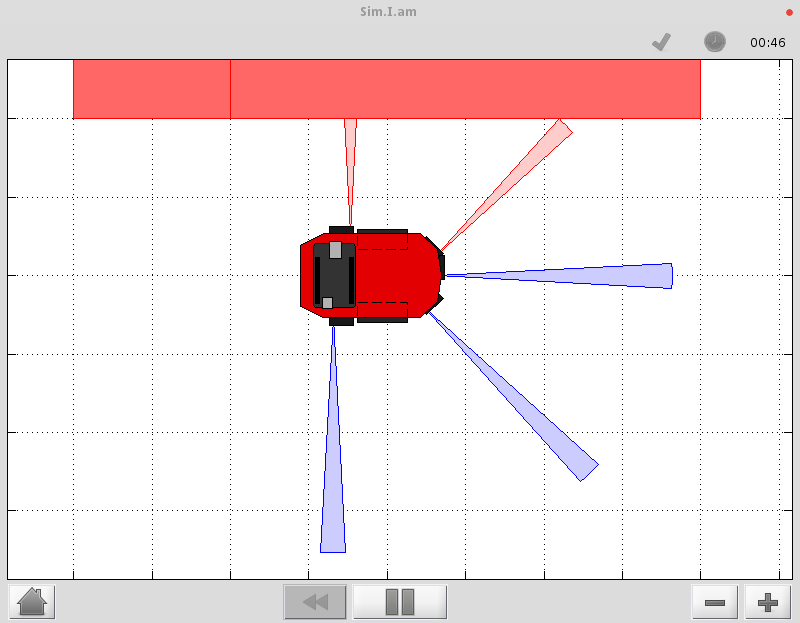
\includegraphics[width=\textwidth]{images/simiam-quickbot.png}
    \caption{Simulated QuickBot}
    \label{fig:simulated-quickbot}
  \end{subfigure}
  \begin{subfigure}{0.45\textwidth}
    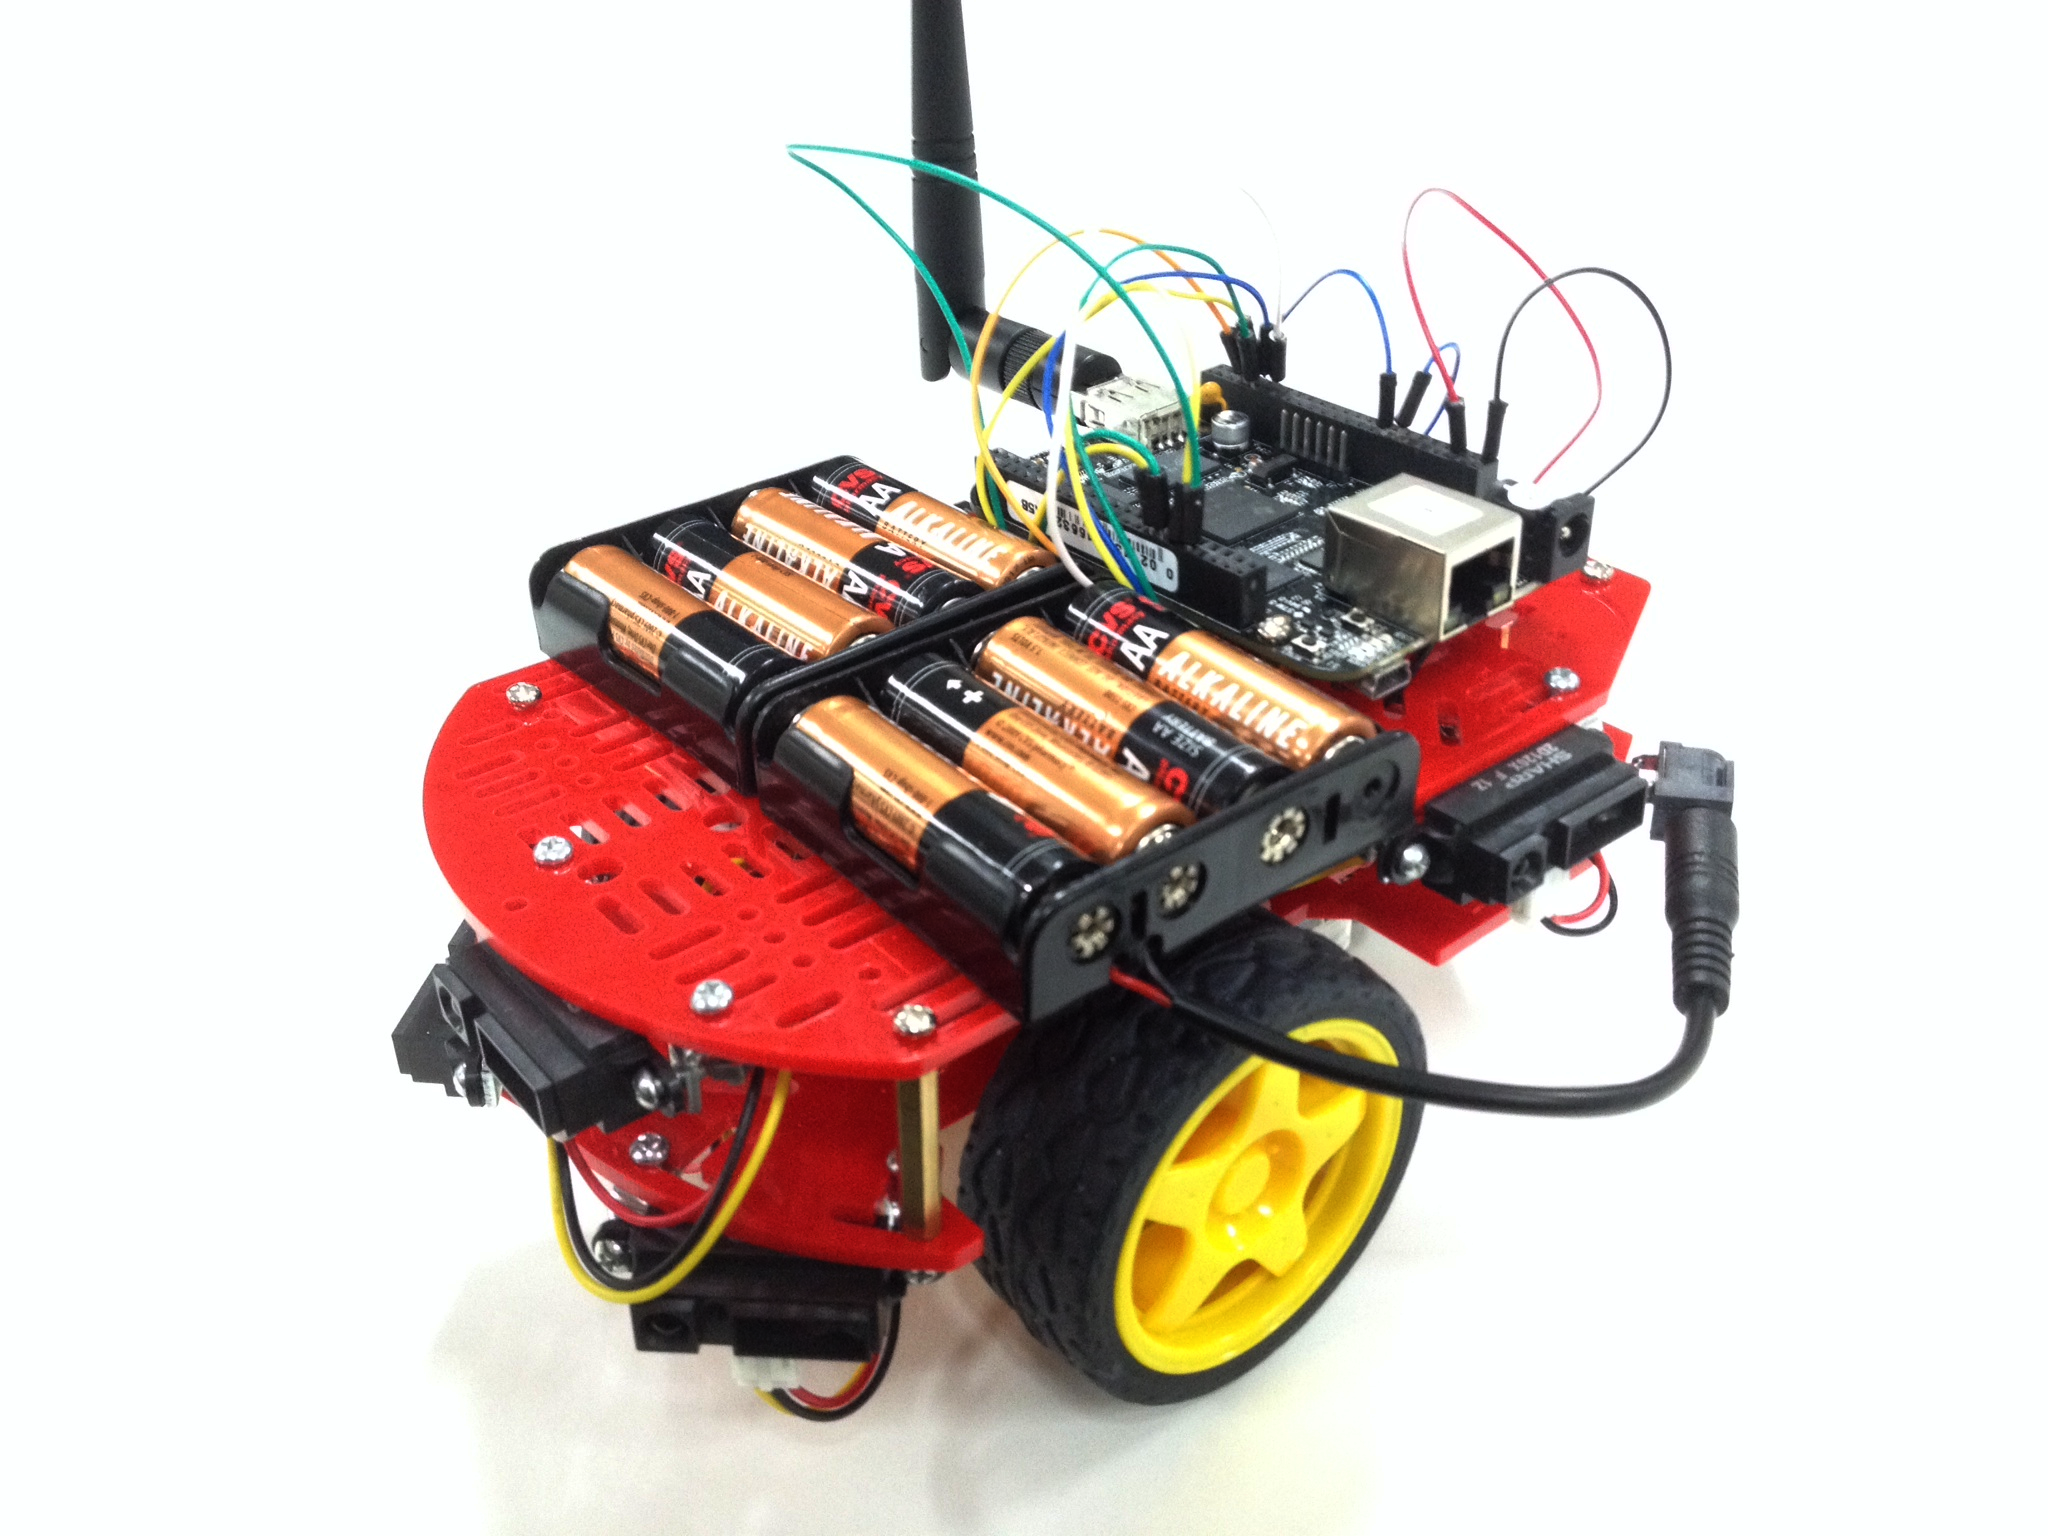
\includegraphics[width=\textwidth]{images/quickbot-red.png}
    \caption{Actual QuickBot}
    \label{fig:actual-quickbot}
  \end{subfigure}
  \caption{The simulated QuickBot and the mobile robot it is based upon.} 
  \label{fig:quickbot}
\end{figure}

Figure \ref{fig:quickbot} shows the simulated and actual QuickBot mobile robot. The robot simulator recreates the QuickBot as faithfully as possible. For example, the range, output, and field of view of the simulated IR range sensors match the specifications in the datasheet for the actual Sharp GP2D120XJ00F infrared proximity sensors on the QuickBot.

\subsection{IR Range Sensors}\label{irprox}
In this section we cover some of the details pertaining to the five simulated IR sensors onboard the simulated QuickBot. 
The orientations (relative to the body of the QuickBot, as shown in Figure \ref{fig:simulated-quickbot}) of IR sensors 1 through 5 are $90^\circ, 45^\circ, 0^\circ$, $-45^\circ$, and $-90^\circ$, respectively. IR range sensors are effective in the range $0.04$ m to $0.3$ m only. However, the IR sensors return raw values in the range of $[0.4,2.75] V$ instead of the measured distances. Figure \ref{fig:ir-volts-meters} demonstrates the function that maps these sensors values to distances. To complicate matters slightly, the BeagleBone Black onboard the physical QuickBot digitizes the analog output voltage using a voltage divider and a 12-bit, 1.8V analog-to-digital converter (ADC). To faithfully recreate the QuickBot in simulation, we simulate the effect of this digitization. Figure \ref{fig:ir-adc} is a look-up table to demonstrate the relationship between the ADC output, the analog voltage from the IR proximity sensor, and the approximate distance that corresponds to this voltage.

\begin{figure}[t]
  \centering
  \begin{subfigure}{0.45\textwidth}
    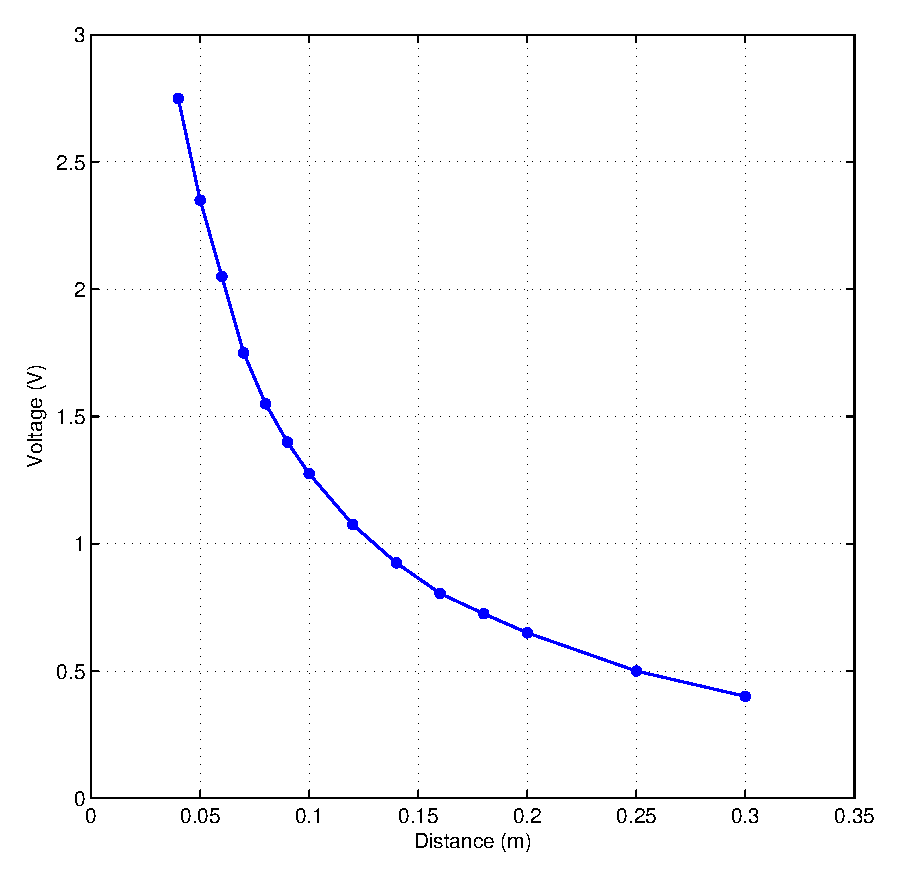
\includegraphics[width=\textwidth]{images/ir-sensor-graph.eps}
    \caption{Analog voltage output when an object is between 0.04m and 0.3m in the IR proximity sensor's field of view.}
    \label{fig:ir-volts-meters}
  \end{subfigure}
  $\qquad$
  \begin{subfigure}{0.45\textwidth}
    \begin{center}
    \begin{tabular}{|p{0.3\textwidth}|p{0.3\textwidth}|p{0.25\textwidth}|}
       \hline
       Distance (m) & Voltage (V) & ADC Out\\
       \hline
       0.04 & 2.750 & 917 \\
       0.05 & 2.350 & 783 \\
       0.06 & 2.050 & 683 \\
       0.07 & 1.750 & 583 \\
       0.08 & 1.550 & 517 \\
       0.09 & 1.400 & 467 \\
       0.10 & 1.275 & 425 \\
       0.12 & 1.075 & 358 \\
       0.14 & 0.925 & 308 \\
       0.16 & 0.805 & 268 \\
       0.18 & 0.725 & 242 \\
       0.20 & 0.650 & 217 \\
       0.25 & 0.500 & 167 \\
       0.30 & 0.400 & 133 \\
       \hline
    \end{tabular}
  \end{center}
    \caption{A look-up table for interpolating a distance (m) from the analog (and digital) output voltages.}
    \label{fig:ir-adc}
  \end{subfigure}
  \caption{A graph and a table illustrating the relationship between the distance of an object within the field of view of an infrared proximity sensor and the analog (and digital) ouptut voltage of the sensor.}
\end{figure}

Any controller can access the IR array through the \texttt{robot} object that is passed into its \texttt{execute} function. For example,
\begin{verbatim}
  ir_distances = robot.get_ir_distances();
  for i=1:numel(robot.ir_array)
    fprintf('IR #%d has a value of %d', i, robot.ir_array(i).get_range());
    fprintf('or %0.3f meters.\n', ir_distances(i));
  end
\end{verbatim}

It is assumed that the function \texttt{get\_ir\_distances} properly converts from the ADC output to an analog output voltage, and then from the analog output voltage to a distance in meters. The conversion from ADC output to analog output voltage is simply

\begin{equation*}
  V_{\text{ADC}} = \left\lfloor\frac{1000\cdot V_{\text{analog}}}{3}\right\rfloor.
\end{equation*}

\textbf{NOTE: For Week 2, the simulator uses a different voltage divider on the ADC; therefore, $V_{\text{ADC}}= V_{\text{analog}}\cdot 1000/2$. This has been fixed in subsequent weeks!}

Converting from the the analog output voltage to a distance is a little bit more complicated, because a) the relationships between analog output voltage and distance is not linear, and b) the look-up table provides a coarse sample of points on the curve in Figure \ref{fig:ir-volts-meters}. MATLAB has a \texttt{polyfit} function to fit a curve to the values in the look-up table, and a \texttt{polyval} function to interpolate a point on that fitted curve. The combination of the these two functions can be use to approximate a distance based on the analog output voltage, and this will be done as part
of the programming assignment in Week 2. 

\subsection{Differential Wheel Drive}\label{diffdrive}
Since the simulated QuickBot has a differential wheel drive (i.e., is not a unicyle), it has to be controlled by specifying the angular velocities of the right and left wheel $(v_r,v_l)$, instead of the linear and angular velocities of a unicycle $(v,\omega)$. These velocities are computed by a transformation from $(v,\omega)$ to $(v_r,v_\ell)$. Recall that the dynamics of the unicycle are defined as
\begin{equation}
 \begin{split}
   \dot{x} &= v\cos(\theta) \\
   \dot{y} &= v\sin(\theta) \\
   \dot{\theta} &= \omega.
 \end{split}
\end{equation}
The dynamics of the differential drive are defined as
\begin{equation}
 \begin{split}
  \dot{x} &= \frac{R}{2}(v_r+v_\ell)cos(\theta) \\
  \dot{y} &= \frac{R}{2}(v_r+v_\ell)sin(\theta) \\
  \dot{\theta} &= \frac{R}{L}(v_r-v_\ell),
 \end{split}
\end{equation}
where $R$ is the radius of the wheels and $L$ is the distance between the wheels.

The speed of the simulated QuickBot can be set in the following way assuming that the \texttt{uni\_to\_diff} function has been implemented, which transforms $(v,\omega)$ to $(v_r,v_\ell)$:
\begin{verbatim}
 v = 0.15; % m/s
 w = pi/4; % rad/s
 % Transform from v,w to v_r,v_l and set the speed of the robot
 [vel_r, vel_l] = obj.robot.dynamics.uni_to_diff(robot,v,w);
 obj.robot.set_speeds(vel_r, vel_l);
\end{verbatim}

The maximum angular wheel velocity for the physical QuickBot is approximately 80 RPM or 8.37 rad/s and this value is reflected in the simulator. It is therefore important to note that if the simulated QuickBot is controlled to move at maximum linear velocity, it is not possible to achieve any angular velocity, because the angular velocity of the wheel will have been maximized. Therefore, there exists a tradeoff between the linear and angular velocity of the QuickBot: \textit{the faster the robot should turn, the slower it has to move forward}.

\subsection{Wheel Encoders}

Each of the wheels is outfitted with a wheel encoder that increments or decrements a tick counter depending on whether the wheel is moving forward or backwards, respectively. Wheel encoders may be used to infer the relative pose of the simulated robot. This inference is called \textbf{odometry}. The relevant information needed for odometry is the radius of the wheel ($32.5$mm), the distance between the wheels ($99.25$mm), and the number of ticks per revolution of the wheel ($16$ ticks/rev). For example,

\begin{verbatim}
 R = robot.wheel_radius; % radius of the wheel
 L = robot.wheel_base_length; % distance between the wheels
 tpr = robot.encoders(1).ticks_per_rev; % ticks per revolution for the right wheel

 fprintf('The right wheel has a tick count of %d\n', robot.encoders(1).state);
 fprintf('The left wheel has a tick count of %d\n', robot.encoders(2).state);
\end{verbatim}

For more information about odometry, see the Week 2 programming assignment.

\newpage
\section{Simulator}

Start the simulator with the \texttt{launch} command in MATLAB from the command window. It is important that this command is executed inside the unzipped folder (but not inside any of its subdirectories).

\begin{figure}[h]
  \centering
  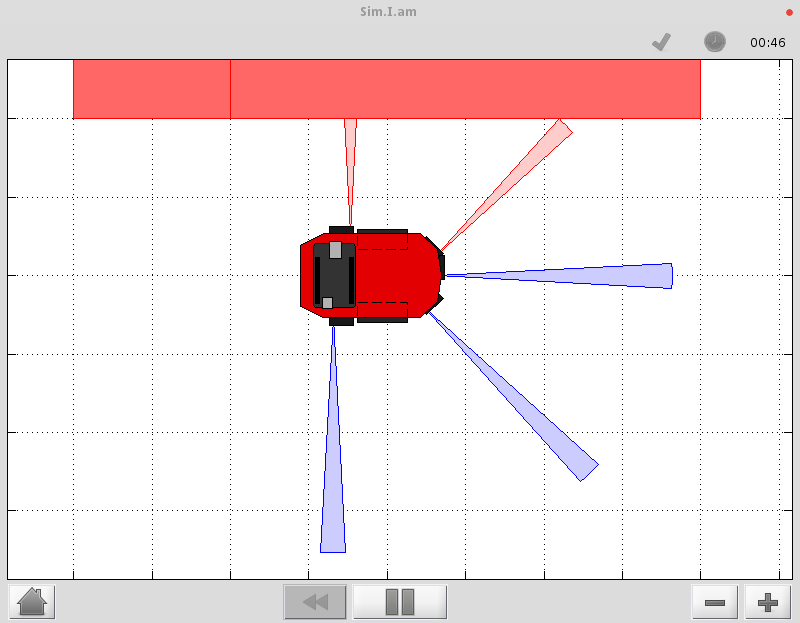
\includegraphics[width=0.45\textwidth]{images/simiam-quickbot.png}
  \caption{\texttt{launch} starts the simulator.}
  \label{fig:simulator}
\end{figure}

Figure \ref{fig:simulator} is a screenshot of the graphical user interface (GUI) of the simulator. The GUI can be controlled by the bottom row of buttons. The first button is the \textit{Home} button and returns you to the home screen. The second button is the \textit{Rewind} button and resets the simulation. The third button is the \textit{Play} button, which can be used to play and pause the simulation. The set of \textit{Zoom} buttons or the mouse scroll wheel allows you to zoom in and out to get a better view of the simulation. Clicking, holding, and moving the mouse allows you to pan around the environment. You can click on a robot to follow it as it moves through the environment.

\newpage
\section{Programming Assignments}

The following sections serve as a tutorial for getting through the simulator portions of the programming exercises. Places where you need to either edit or add code are marked off by a set of comments. For example,

\begin{verbatim}
  %% START CODE BLOCK %%
    [edit or add code here]
  %% END CODE BLOCK %%
\end{verbatim}

To start the simulator with the \texttt{launch} command from the command window, it is important that this command is executed inside the unzipped folder (but not inside any of its subdirectories).

\subsection{Week 1}

This week's exercises will help you learn about MATLAB and robot simulator. \textbf{If you do not already have access to MATLAB, a student license will be made available to registered participants of this course starting in Week 2. You can easily put off the optional Week 1 MATLAB assignment until Week 2 without falling behind.} 

\begin{enumerate}
\item Install the GUI Layout Toolbox using the instructions provided in the \emph{Preparing for Programming Assignments} page under \emph{Week 1}. 
\item Familiarize yourself with the simulator by reading this manual and downloading the robot simulator posted on the \textit{Optional Programming Assignment 1: Instructions} section under \emph{Week 1}.
\item Start the simulator by running the \texttt{launch} command from the command window. If the GUI Layout Toolbox has been installed correctly (instructions for this can be found in the \emph{Preparing for Programming Assignments} page under \emph{Week 1}), the home screen should appear. Pressing the Play button will then show a robot which is stationary (it will move once we design controllers for it next week!). 
\end{enumerate}

\newpage
\subsection{Week 2}
\label{sec:week-2}
\textbf{If you are installing MATLAB this week, follow the instructions on the page titled \emph{Installing MATLAB} under Week 2 first. Then return to Week 1's assignment (above) before completing this week.} 

Start by downloading the robot simulator for this week from the Week 2 programming assignment. Before you can design and test controllers in the simulator, you will need to implement three components of the simulator:

\begin{enumerate}
 \item Implement the transformation from unicycle dynamics to differential drive dynamics, i.e. convert from $(v,\omega)$ to the right and left \textbf{angular} wheel speeds $(v_r,v_l)$.
 
 In the simulator, $(v,\omega)$ corresponds to the variables \texttt{v} and \texttt{w}, while $(v_r,v_l)$ correspond to the variables \texttt{vel\_r} and \texttt{vel\_l}. The function used by the controllers to convert from unicycle dynamics to differential drive dynamics is located in \texttt{+simiam/+robot/+dynamics/DifferentialDrive.m}. The function is named \texttt{uni\_to\_diff}, and inside of this function you will need to define \texttt{vel\_r} ($v_r$) and \texttt{vel\_l} ($v_l$) in terms of \texttt{v}, \texttt{w}, \texttt{R}, and \texttt{L}. \texttt{R} is the radius of a wheel, and \texttt{L} is the distance separating the two wheels. Make sure to refer to Section \ref{diffdrive} on ``Differential Wheel Drive'' for the dynamics.
 
 \item Implement odometry for the robot, such that as the robot moves around, its pose $(x,y,\theta)$ is estimated based on how far each of the wheels have turned. Assume that the robot starts at (0,0,0).
 
 The tutorial located at \url{www.orcboard.org/wiki/images/1/1c/OdometryTutorial.pdf} covers how odometry is computed. The general idea behind odometry is to use wheel encoders to measure the distance the wheels have turned over a small period of time, and use this information to approximate the change in pose of the robot.

 The pose of the robot is composed of its position $(x,y)$ and its orientation $\theta$ on a 2 dimensional plane (\textbf{note}: the video lecture may refer to robot's orientation as $\phi$). The currently estimated pose is stored in the variable \texttt{state\_estimate}, which bundles \texttt{x} ($x$), \texttt{y} ($y$), and \texttt{theta} ($\theta$). The robot updates the estimate of its pose by calling the \texttt{update\_odometry} function, which is located in \texttt{+simiam/+controller/+quickbot/QBSupervisor.m}. This function is called every \texttt{dt} seconds, where \texttt{dt} is $0.033$s (or a little more if the simulation is running slower).
 \begin{verbatim}  
  % Get wheel encoder ticks from the robot
  right_ticks = obj.robot.encoders(1).ticks;
  left_ticks = obj.robot.encoders(2).ticks;

  % Recall the wheel encoder ticks from the last estimate
  prev_right_ticks = obj.prev_ticks.right;
  prev_left_ticks = obj.prev_ticks.left;

  % Previous estimate 
  [x, y, theta] = obj.state_estimate.unpack();

  % Compute odometry here
  R = obj.robot.wheel_radius;
  L = obj.robot.wheel_base_length;
  m_per_tick = (2*pi*R)/obj.robot.encoders(1).ticks_per_rev;\end{verbatim}
  The above code is already provided so that you have all of the information needed to estimate the change in pose of the robot. \texttt{right\_ticks} and \texttt{left\_ticks} are the accumulated wheel encoder ticks of the right and left wheel. \texttt{prev\_right\_ticks} and \texttt{prev\_left\_ticks} are the wheel encoder ticks of the right and left wheel saved during the last call to \texttt{update\_odometry}. \texttt{R} is the radius of each wheel, and \texttt{L} is the distance separating the two wheels. \texttt{m\_per\_tick} is a constant that tells you how many meters a wheel covers with each tick of the wheel encoder. So, if you were to multiply \texttt{m\_per\_tick} by (\texttt{right\_ticks}-\texttt{prev\_right\_ticks}), you would get the distance travelled by the right wheel since the last estimate.
  
  Once you have computed the change in $(x,y,\theta)$ (let us denote the changes as \texttt{x\_dt}, \texttt{y\_dt}, and \texttt{theta\_dt}) , you need to update the estimate of the pose:
  \begin{verbatim}
    theta_new = theta + theta_dt;
    x_new = x + x_dt;
    y_new = y + y_dt;\end{verbatim}
 
 \item Read the "IR Range Sensors" section in the manual and take note of the table in Figure \ref{fig:ir-adc}, which maps distances (in meters) to raw IR values. Implement code that converts raw IR values to distances (in meters).
 
 To retrieve the distances (in meters) measured by the IR proximity sensor, you will need to implement a conversion from the raw IR values to distances in the \texttt{get\_ir\_distances} function located in \texttt{+simiam/+robot/Quickbot.m}.
 \begin{verbatim}
  function ir_distances = get_ir_distances(obj)
      ir_array_values = obj.ir_array.get_range();
      ir_voltages = ir_array_values;
      coeff = [];
      ir_distances = polyval(coeff, ir_voltages);
  end\end{verbatim}
  The variable \texttt{ir\_array\_values} is an array of the IR raw values. Divide this array by $500$ to compute the \texttt{ir\_voltages} array. The \texttt{coeff} should be the coefficients returned by
  \begin{verbatim}
    coeff = polyfit(ir_voltages_from_table, ir_distances_from_table, 5);\end{verbatim}
where the first input argument is an array of IR voltages from the table in Figure \ref{fig:ir-adc} and the second argument is an array of the corresponding distances from the table in Figure \ref{fig:ir-adc}. The third argument specifies that we will use a fifth-order polynomial to fit to the data. Instead of running this fit every time, execute the polyfit once in the MATLAB command line, and enter them manually on the third line, i.e. \texttt{coeff = [ ... ];}. If the coefficients are properly computed, then the last line will use polyval to convert from IR voltages to distances using a fifth-order polynomial using the coefficients in \texttt{coeff}. 
 
\end{enumerate}

\subsubsection*{How to test it all}

To test your code, the simulator is set to run a single P-regulator that will steer the robot to a particular angle (denoted $\theta_d$ or, in code, \texttt{theta\_d}). This P-regulator is implemented in \texttt{+simiam/+controller/} \texttt{GoToAngle.m}. If you want to change the linear velocity of the robot, or the angle to which it steers, edit the following two lines in \texttt{+simiam/+controller/+quickbot/QBSupervisor.m}
 \begin{verbatim}
  obj.theta_d = pi/4;
  obj.v = 0.1; %m/s\end{verbatim}
\begin{enumerate}
  \item To test the transformation from unicycle to differential drive, first set \texttt{obj.theta\_d=0}. The robot should drive straight forward. Now, set \texttt{obj.theta\_d} to positive or negative $\frac{\pi}{4}$. If positive, the robot should start off by turning to its left, if negative it should start off by turning to its right. \textbf{Note}: If you haven't implemented odometry yet, the robot will just keep on turning in that direction.
  \item To test the odometry, first make sure that the transformation from unicycle to differential drive works correctly. If so, set \texttt{obj.theta\_d} to some value, for example $\frac{\pi}{4}$, and the robot's P-regulator should steer the robot to that angle. You may also want to uncomment the \texttt{fprintf} statement in the \texttt{update\_odometry} function to print out the current estimate position to see if it make sense. Remember, the robot starts at $(x,y,\theta)=(0,0,0)$.
  \item To test the IR raw to distances conversion, edit \texttt{+simiam/+controller/}\texttt{GoToAngle.m} and uncomment the following section:
  \begin{verbatim}
  % for i=1:numel(ir_distances)
  %   fprintf('IR %d: %0.3fm\n', i, ir_distances(i));
  % end\end{verbatim}
  This \texttt{for} loop will print out the IR distances. If there are no obstacles (for example, walls) around the robot, these values should be close (if not equal to) $0.3$m. Once the robot gets within range of a wall, these values should decrease for some of the IR sensors (depending on which ones can sense the obstacle). \texttt{Note:} The robot will eventually collide with the wall, because we have not designed an obstacle avoidance controller yet!
\end{enumerate}

\end{document}
